% Para funcionar as pausas, basta retirar o [handout] do document class:
% \documentclass{beamer}
\documentclass[handout]{beamer}
\usetheme{CambridgeUS}
\usecolortheme{seagull}
\usepackage[sort, numbers]{natbib}
% \usepackage{biblatex}
%\newcommand{\newblock}{}
\usepackage[english]{babel}
\usepackage[latin1]{inputenc}
\usepackage[T1]{fontenc}
%\usepackage[portuguese, algoruled, longend, linesnumbered, noline]{algorithm2e}
\usepackage{subfigure}
\usepackage{graphicx}
\usepackage{epstopdf}
\usepackage{multimedia}
\usepackage{tikz}
\usepackage{pgfgantt}
\usepackage{subfigure}

\title[Coverage based debugging visualization]{Coverage based debugging
visualization} \author[Danilo Mutti]{Danilo Mutti\\ Adviser: Prof. Marcos
Lordello Chaim, Ph.D.} \institute[EACH-USP]{Software Analysis \& Experimentation Group
--- SAEG\\
School of Arts, Sciences and Humanities\\
University of Sao Paulo}

\setbeamercovered{transparent}

\begin{document}

\begin{frame}[plain]
\titlepage
\end{frame}

\begin{frame}{Agenda}
\tableofcontents
\end{frame}

\section{Introduction}

\begin{frame}
    \sectionpage
\end{frame}

\begin{frame}[allowframebreaks]{Motivation}
    \begin{itemize}
        \item Debugging is an expensive, ad-hoc manual process~\cite{jones2007}.
        \item Estimated global cost US\$ 312 billion a year~\cite{britton2013reversible}.
        \item Coverage based debugging techniques utilizes coverage information
        of code components:
            \begin{itemize}
                \item statements;
                \item predicates;
                \item def-use associations;
                \item call functions.
            \end{itemize}
        \framebreak
        \item Heuristics are used to assign suspiciousness values to statements;
        \item What is the best strategy to display it?
        \item Current visualization techniques does not provide context!
        \item Additional contextual information might leverage developers'
        performance~\cite{parnin2011automated}.
    \end{itemize}
\end{frame}

\begin{frame}{Objectives}
    \begin{itemize}
        \item Develop a novel 3D metaphor to represent suspiciousness
        information obtained from coverage based debugging techniques.
        \item Explore how to adequately display larger entities of programs and
        their suspiciousness values.
        \item Embed the new metaphor as a plug-in into a IDE.
        \item Add contextual information to support fault
        localization~\cite{souza13adding}.
        \item Plan and execute an experiment.
    \end{itemize}
\end{frame}

\section{Background}

\begin{frame}
    \sectionpage
\end{frame}

\begin{frame}{First computer bug}
    \begin{figure}
        \includegraphics[width=.7\linewidth]{../figures/firstbug}
    \end{figure}
\end{frame}

\begin{frame}{Bugs Everywhere}
    \begin{itemize}
        \item Lines of code, program state, and execution output are elements
            \begin{itemize}
                \item interconnected;
                \item separated not only in space but also in time.
            \end{itemize}
        \item According to Zeller~\cite{zeller2009programs}:
        \begin{itemize}
            \item a defect denotes an incorrect program code;
            \item an infection denotes an incorrect program state;
            \item a failure denotes an observable incorrect program behavior.
        \end{itemize}
        \item Defect is more appealing term than bug.
    \end{itemize}
\end{frame}

\begin{frame}{Code Coverage}
    \begin{itemize}
        \item Also known as program spectra.
        \item The set of components covered during the execution of test
        cases~\cite{elbaum2001}.
        \begin{itemize}
            \item components: statements, predicates, def-use associations or
            function calls~\cite{Abreu2008};
            \item coverages obtained by testing the unit of the program.
        \end{itemize}
        \item \textit{MethodCallPair} (MCP) are coverages obtained from
        integration testing data.
    \end{itemize}
\end{frame}

\begin{frame}[allowframebreaks]{Coverage Based Debugging}

    \begin{itemize}
        \item Code coverage information is utilized by heuristics (e.g:
        TARANTULA~\cite{jones2002visualization}) to calculate the suspiciousness
        of components. \begin{equation}H_{T} = \frac{\frac{c_{ef}}{c_{ef} +
        c_{nf}}}{\frac{c_{ef}}{c_{ef} + c_{nf}} + \frac{c_{ep}}{c_{ep} +
        c_{np}}} \end{equation}
        \item After assigning a suspiciousness value to these components, it
        generates a descending list of components, ordered by suspiciousness.
        \item Current ranking heuristics lack guidance to search for faults in
        larger portions of code. They assign suspiciousness values only to
        statements!
        \framebreak
        \item Contextual guidance might be helpful to coverage based
        debugging~\cite{parnin2011automated}.
        \item Souza~\cite{souza2012depuracao} proposed:
        \begin{itemize}
            \item Code hierarchy (CH), which attributes suspiciousness values to
            packages, classes and methods. Represented by a pair (\textit{susp},
            \textit{number}).
            \item Roadmaps from the ranking of the MCP coverage (R-MCP).
        \end{itemize}
    \end{itemize}

\end{frame}

\begin{frame}[allowframebreaks]{Information Visualization}

    \begin{itemize}
        \item Mapping of data to pixel values in such a way that meaningful
        conclusions about the data can be drawn~\cite{erik2008color}.
        \item Visual information, when well organized and arranged in a
        structured way, is capable of elevating our comprehension levels about
        some information.
        \item It is more effective to use colors, shapes and textures to convey
        information when compared to a text-only approach.
        \framebreak
        \item Metaphors: a fundamental part of our conceptual system of thought
        and action.
        \item HCI + Metaphors
        \begin{itemize}
            \item A cross-domain mapping, with the goal of allowing the
            transference of knowledge from a source domain to a target domain.
            \item To give users instantaneous knowledge about how to interact
            with the user interface.
        \end{itemize}
    \end{itemize}

\end{frame}

\begin{frame}{Visual Encoding -- Preattentive Attributes}
    \begin{figure}
        \includegraphics[width=.8\linewidth]{../figures/ali-encodings}
    \end{figure}
\end{frame}

\begin{frame}{Software Visualization}

    \begin{itemize}
        \item The visualization of artifacts related to software and its
        development process.
        \item Artifacts -- design documentation, changes in the source code, bug
        reports and coverage based debugging information.
        \item To visualize the structure, behavior, and evolution of software.
        \item It is important to follow at least one of the following
        principles:
        \begin{itemize}
            \item \textit{interactive exploration} -- allows the user to
            first get an overview, and then zoom and filter, getting the details on demand;
            \item \textit{focus $+$ context} -- provides both an overview
            and detail at the same time.
        \end{itemize}
    \end{itemize}
\end{frame}

\section{Related Work}

\begin{frame}
    \sectionpage
\end{frame}

\begin{frame}{2D Visualization}
    \begin{itemize}
        \item Largely explored.
        \item It poses almost no challenge for the regular user.
        \item Mouse and keyboard.
        \item Three major groups:
        \begin{itemize}
            \item Seesoft.
            \item Treemaps.
            \item Graphs.
        \end{itemize}
    \end{itemize}
\end{frame}

\begin{frame}{2D -- Seesoft}
    \begin{figure}
    \includegraphics[width=.54\textwidth]{../figures/eick1992seesoft}
    \end{figure}
\end{frame}

\begin{frame}{2D -- Treemaps}
    \begin{figure}
    \includegraphics[width=.7\textwidth]{../figures/shneiderman1992tree}
    \end{figure}
\end{frame}

\begin{frame}{2D -- Graphs}
    \begin{figure}
    \includegraphics[width=.55\textwidth]{../figures/zaninotto2013codeflowers}
    \end{figure}
\end{frame}

\begin{frame}{3D Visualization}
    \begin{itemize}
        \item Recent popularity due to:
        \begin{itemize}
            \item Low cost/high-performance graphical processing units.
            \item Several options of 3D rendering frameworks.
        \end{itemize}
        \item Two major groups:
        \begin{itemize}
            \item Botanical trees.
            \item Cities.
        \end{itemize}
    \end{itemize}
\end{frame}

\begin{frame}{3D -- Botanical Trees}
    \begin{figure}
    \includegraphics[width=\textwidth]{../figures/erra2012towards}
    \end{figure}
\end{frame}

\begin{frame}{3D -- Cities}
    \begin{figure}
    \includegraphics[width=.95\textwidth]{../figures/wettel2007program}
    \end{figure}
\end{frame}

\section{CodeForest}

\begin{frame}
    \sectionpage
\end{frame}

\begin{frame}{CodeForest -- Metaphor}
    \begin{itemize}
        \item Every class is represented as a cactus.
        \item A branch is drawn in the cactus for every method within a class.
        \item Thorns are associated with nodes.
        \item Position, color, size and thickness of every cactus of the forest
        is determined by its suspiciousness value.
        \item The higher the score, the redder, taller, thicker and rightmost is
        the cactus.
        \item High ranked branches are closer to the ground.
        \item High ranked thorns are closer to the trunk.
     \end{itemize}
\end{frame}

\begin{frame}{Cactus}
    \begin{figure}
        \centering
        \includegraphics[height=7cm]{../figures/internal_metaphor}
    \end{figure}
\end{frame}

\begin{frame}{Cacti Forest}
    \begin{figure}
        \includegraphics[width=.95\textwidth]{../figures/metaphor}
    \end{figure}
\end{frame}

\begin{frame}{CodeForest -- Plug-in}
    \begin{itemize}
        \item Built
        \begin{itemize}
            \item using Java, Java3D;
            \item atop the Eclipse Platform (OSGi);
            \item \url{https://github.com/saeg/code-forest}
        \end{itemize}
        \item The plug-in provides:
        \begin{itemize}
            \item an implementation of the metaphor, a virtual 3D forest;
            \item filtering tools (text and score);
            \item a roadmap;
            \item an improved Java editor.
        \end{itemize}
        \item Depends on the Integration Coverage-based Debugging (ICD)
        tool~\cite{souza13adding, souza2012depuracao} and the Instrumentation
        Strategies Simulator (InSS)~\cite{souza2012depuracao}.
     \end{itemize}
\end{frame}

\begin{frame}{Eclipse Plug-in I}
    \begin{figure}
        \centering
        \includegraphics[width=\linewidth]{../figures/commons_math_complex_04_view_max}
    \end{figure}
\end{frame}

\begin{frame}{Eclipse Plug-in II}
    \begin{figure}
        \centering
        \includegraphics[width=\linewidth]{../figures/commons_math_complex_02_red_green_grey}
    \end{figure}
\end{frame}

\begin{frame}{Eclipse Plug-in III}
    \begin{figure}
        \centering
        \includegraphics[width=\linewidth]{../figures/commons_math_complex_05_view_min}
    \end{figure}
\end{frame}

\begin{frame}{ICD Implementation}
    \begin{figure}
        \centering
        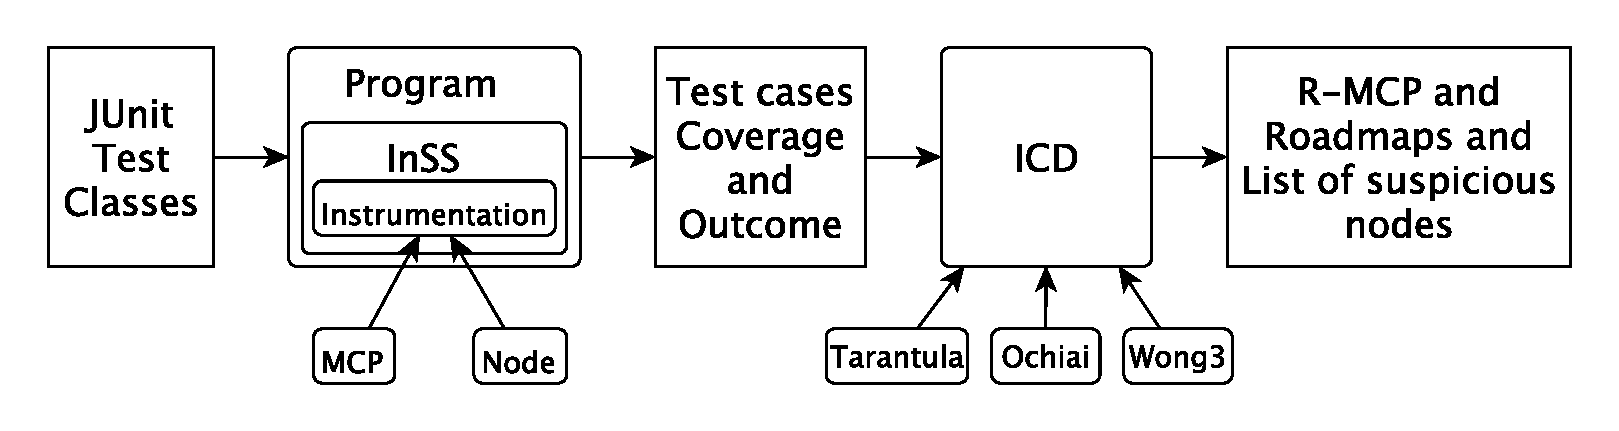
\includegraphics[width=\textwidth]{../figures/icd_implementation}
    \end{figure}
\end{frame}

\section{Experimentation}

\begin{frame}
    \sectionpage
\end{frame}

\begin{frame}[allowframebreaks]{Experimental Design}
    \begin{itemize}
        \item Research questions
            \begin{itemize}
                \item Is the metaphor adequate to the problem of locating
                defects?
                \item Are the tools embedded within the plug-in useful?
                \item What is the dynamics between the developer and the
                tool when he/she is trying to locate defects?
            \end{itemize}
        \item In the experiment, every participant received two tasks:
            \begin{itemize}
                \item Apache Commons-Math.
                \item Thoughtworks XStream.
            \end{itemize}
        \framebreak
        \item Participants received a 30-minute training session before starting
        the experiment.
        \item They had 60 minutes to execute the first task of the experiment
        and 30 minutes to execute the following task.
        \item Every experiment resulted in:
        \begin{itemize}
            \item A log file, containing all actions performed.
            \item Two locations in the source code, one for each defect.
            \item A questionnaire (26 questions) filled at the end of
            experiment.
        \end{itemize}
        \item The machine utilized was a MacBook Pro with a 17-inch secondary
        display.
    \end{itemize}
\end{frame}

\begin{frame}{Pilot Experiment}
    \begin{itemize}
        \item The pilot experiment helped us to trim off the edges from the
        plug-in.
        \item The initial version had two implementations of the 3D
        forest environment: mouse and keyboard.
        \begin{itemize}
            \item Participant \#1 disliked the mouse-operated version,
            motivating us to discontinue it before making new experiments.
        \end{itemize}
        \item It displayed the whole codebase as a forest, regardless whether
        elements were exercised by tests or not.
        \begin{itemize}
            \item The forest was a faithful representation of the codebase,
            but too slow to manipulate.
            \item The great number of elements in the scene draw away the user's
            attention.
        \end{itemize}
    \end{itemize}
\end{frame}

\begin{frame}{Experiments I}
    \begin{itemize}
        \item The participants are part of the Software Analysis \&
        Experimentation Group (SAEG), with distinct profiles:
            \begin{itemize}
                \item 1 -- A Master's student, with one year of professional
                experience.
                \item 2 -- A Master's student with a bachelor's degree in
                Applied Mathematics, and no experience at all.
                \item 3 -- An undergraduate student in Information Systems with
                good, though not industrial, coding skills in Java and JUnit.
                \item 4 -- A Master's student with an Information Systems
                diploma, 6+ years of experience; proficient in Java.
            \end{itemize}
    \end{itemize}
\end{frame}

\begin{frame}{Experiments II - Participant \#1}
        \begin{figure}
            \includegraphics[width=.5\textwidth]{figures/pilot_experiment}
        \end{figure}
\end{frame}

\begin{frame}{Experiments III - Participant \#2}
        \begin{figure}
            \includegraphics[width=.5\textwidth]{figures/experiment_1}
        \end{figure}
\end{frame}

\begin{frame}{Experiments IV - Participant \#3}
        \begin{figure}
            \includegraphics[width=.5\textwidth]{figures/experiment_2}
        \end{figure}
\end{frame}

\begin{frame}{Experiments V - Participant \#4}
        \begin{figure}
            \includegraphics[width=.5\textwidth]{figures/experiment_3}
        \end{figure}
\end{frame}

\begin{frame}{Experiments VI}
    \begin{itemize}
        \item Overall opinion about the plug-in was positive. However, the way
        users explore the forest and the strategy of positioning branches
        should be reviewed.
        \item Threats to validity:
            \begin{itemize}
                \item We performed an exploratory experiment, which limits the
                range of our findings.
                \item All participants are part of the same research group,
                which could introduce bias into our results.
            \end{itemize}
    \end{itemize}
\end{frame}

\section{Conclusions, Contributions and Future Work}

\begin{frame}
    \sectionpage
\end{frame}

\begin{frame}{Conclusions}
    \begin{itemize}
        \item Several visualizations have been proposed in the last 40 years,
        but most of them are poorly suited to the task of debugging.
        \item There is a global need for better debugging tools. Global cost of
        debugging is estimated to orbitate around US\$ 312
        billion~\cite{britton2013reversible}.
        \item Our metaphor maps classes into cacti, methods into branches, and
        lines of code into thorns.
        \item Our experiment showed that
            \begin{itemize}
                \item every participant utilized the CodeForest;
                \item users with low or no experience utilized the roadmap
                together with the virtual 3D environment to investigate the
                defect;
                \item experienced users utilized the roadmap.
            \end{itemize}
    \end{itemize}
\end{frame}

\begin{frame}{Contributions}
    \begin{itemize}
        \item A thorough literature review of 2D and 3D methods to visualize
        software data.
        \item A fully functional prototype utilized to perform experiments and produce results.
        \item A plug-in targeted to the Eclipse IDE that serves as the
        foundation of a system to explore other debugging techniques.
        \item An exploratory, qualitative experiment to assess the adequacy of
        the CodeForest metaphor in the activity of investigating defects.
    \end{itemize}
\end{frame}

\begin{frame}{Future Work}
    \begin{itemize}
        \item Perform a quantitative experiment, with different groups of
        developers.
        \item Improve the training sessions; one for each topic: debugging
        techniques, JUnit, Eclipse, and the CodeForest plug-in.
        \item Utilize Apache Lucene to deliver better textual search.
        \item Migrate to a better, more advanced 3D engine.
        \item Complete the integration with the ICD/InSS toolset.
    \end{itemize}
\end{frame}

\section{References}

\begin{frame}
    \sectionpage
\end{frame}

\begin{frame}[allowframebreaks]{References}
\bibliographystyle{unsrtnat}
\bibliography{daniloApresentacao}
\end{frame}

\end{document}